%% abtex2-modelo-trabalho-academico.tex, v-1.9.7 laurocesar
%% Copyright 2012-2018 by abnTeX2 group at http://www.abntex.net.br/ 
%%
%% This work may be distributed and/or modified under the
%% conditions of the LaTeX Project Public License, either version 1.3
%% of this license or (at your option) any later version.
%% The latest version of this license is in
%%   http://www.latex-project.org/lppl.txt
%% and version 1.3 or later is part of all distributions of LaTeX
%% version 2005/12/01 or later.
%%
%% This work has the LPPL maintenance status `maintained'.
%% 
%% The Current Maintainer of this work is the abnTeX2 team, led
%% by Lauro César Araujo. Further information are available on 
%% http://www.abntex.net.br/
%%
%% This work consists of the files abntex2-modelo-trabalho-academico.tex,
%% abntex2-modelo-include-comandos and abntex2-modelo-references.bib
%%

% ------------------------------------------------------------------------
% ------------------------------------------------------------------------
% abnTeX2: Modelo de Trabalho Academico (tese de doutorado, dissertacao de
% mestrado e trabalhos monograficos em geral) em conformidade com 
% ABNT NBR 14724:2011: Informacao e documentacao - Trabalhos academicos -
% Apresentacao
% ------------------------------------------------------------------------
% ------------------------------------------------------------------------

\documentclass[
	% -- opções da classe memoir --
	12pt,				% tamanho da fonte
	openright,			% capítulos começam em pág ímpar (insere página vazia caso preciso)
	twoside,			% para impressão em recto e verso. Oposto a oneside
	a4paper,			% tamanho do papel. 
	% -- opções da classe abntex2 --
	%chapter=TITLE,		% títulos de capítulos convertidos em letras maiúsculas
	%section=TITLE,		% títulos de seções convertidos em letras maiúsculas
	%subsection=TITLE,	% títulos de subseções convertidos em letras maiúsculas
	%subsubsection=TITLE,% títulos de subsubseções convertidos em letras maiúsculas
	% -- opções do pacote babel --
	english,			% idioma adicional para hifenização
	french,				% idioma adicional para hifenização
	spanish,			% idioma adicional para hifenização
	brazil				% o último idioma é o principal do documento
	]{abntex2}

% ---
% Pacotes básicos 
% ---
\usepackage{lmodern}			% Usa a fonte Latin Modern			
\usepackage[T1]{fontenc}		% Selecao de codigos de fonte.
\usepackage[utf8]{inputenc}		% Codificacao do documento (conversão automática dos acentos)
\usepackage{indentfirst}		% Indenta o primeiro parágrafo de cada seção.
\usepackage{color}				% Controle das cores
\usepackage{graphicx}			% Inclusão de gráficos
\usepackage{microtype} 			% para melhorias de justificação
% ---
		
% ---
% Pacotes adicionais, usados apenas no âmbito do Modelo Canônico do abnteX2
% ---
\usepackage{lipsum}				% para geração de dummy text
% ---

% ---
% Pacotes de citações
% ---
\usepackage[brazilian,hyperpageref]{backref}	 % Paginas com as citações na bibl
\usepackage[alf]{abntex2cite}	% Citações padrão ABNT

% --- 
% CONFIGURAÇÕES DE PACOTES
% --- 

% ---
% Configurações do pacote backref
% Usado sem a opção hyperpageref de backref
\renewcommand{\backrefpagesname}{Citado na(s) página(s):~}
% Texto padrão antes do número das páginas
\renewcommand{\backref}{}
% Define os textos da citação
\renewcommand*{\backrefalt}[4]{
	\ifcase #1 %
		Nenhuma citação no texto.%
	\or
		Citado na página #2.%
	\else
		Citado #1 vezes nas páginas #2.%
	\fi}%
% ---

% ---
% Informações de dados para CAPA e FOLHA DE ROSTO
% ---
\titulo{PIM V \\ Projeto Integrado Multidiciplinar V}
\autor{Pedro José Laurenti de Matos (RA:0621134)\\
Cleverson da Silva Souza (RA: 0620885)\\
Luiz Gustavo Nascimento de Souza (RA: 0618130)\\
Fernando de Sampaio Steimback Vidal (RA: 0626729)\\
Larissa Tamires de Araujo Nascimento (RA: 0622906)\\
} %falta%
\local{Brasil}
\data{Março de 2023}
\orientador{Davi Lazer Grave Teixeira
de Andrade} %falta%
\instituicao{
  Universidade Paulista -- UNIP
  \par
  Curso de Análise e Desenvolvimento de Sistemas
  \par
  Programa de Pós-Graduação}
\tipotrabalho{Trabalho Científico}
% O preambulo deve conter o tipo do trabalho, o objetivo, 
% o nome da instituição e a área de concentração 
\preambulo{Trabalho científico produzido para colocar em prática as habilidades adquiridas no segundo período do curso de Análise e Desenvolvimento de Sistemas.}
% ---


% ---
% Configurações de aparência do PDF final

% alterando o aspecto da cor azul
\definecolor{blue}{RGB}{41,5,195}

% informações do PDF
\makeatletter
\hypersetup{
     	%pagebackref=true,
		pdftitle={\@title}, 
		pdfauthor={\@author},
    	pdfsubject={\imprimirpreambulo},
	    pdfcreator={LaTeX with abnTeX2},
		pdfkeywords={abnt}{latex}{abntex}{abntex2}{trabalho acadêmico}, 
		colorlinks=true,       		% false: boxed links; true: colored links
    	linkcolor=blue,          	% color of internal links
    	citecolor=blue,        		% color of links to bibliography
    	filecolor=magenta,      		% color of file links
		urlcolor=blue,
		bookmarksdepth=4
}
\makeatother
% --- 

% ---
% Posiciona figuras e tabelas no topo da página quando adicionadas sozinhas
% em um página em branco. Ver https://github.com/abntex/abntex2/issues/170
\makeatletter
\setlength{\@fptop}{5pt} % Set distance from top of page to first float
\makeatother
% ---

% ---
% Possibilita criação de Quadros e Lista de quadros.
% Ver https://github.com/abntex/abntex2/issues/176
%
\newcommand{\quadroname}{Quadro}
\newcommand{\listofquadrosname}{Lista de quadros}

\newfloat[chapter]{quadro}{loq}{\quadroname}
\newlistof{listofquadros}{loq}{\listofquadrosname}
\newlistentry{quadro}{loq}{0}

% configurações para atender às regras da ABNT
\setfloatadjustment{quadro}{\centering}
\counterwithout{quadro}{chapter}
\renewcommand{\cftquadroname}{\quadroname\space}
\renewcommand*{\cftquadroaftersnum}{\hfill--\hfill}

\setfloatlocations{quadro}{hbtp} % Ver https://github.com/abntex/abntex2/issues/176
% ---

% --- 
% Espaçamentos entre linhas e parágrafos 
% --- 

% O tamanho do parágrafo é dado por:
\setlength{\parindent}{1.3cm}

% Controle do espaçamento entre um parágrafo e outro:
\setlength{\parskip}{0.2cm}  % tente também \onelineskip

% ---
% compila o indice
% ---
\makeindex
% ---

% ----
% Início do documento
% ----
\begin{document}

% Seleciona o idioma do documento (conforme pacotes do babel)
%\selectlanguage{english}
\selectlanguage{brazil}

% Retira espaço extra obsoleto entre as frases.
\frenchspacing 

% ----------------------------------------------------------
% ELEMENTOS PRÉ-TEXTUAIS
% ----------------------------------------------------------
% \pretextual

% ---
% Capa
% ---
\imprimircapa
% ---

% ---
% Folha de rosto
% (o * indica que haverá a ficha bibliográfica)
% ---
\imprimirfolhaderosto*
% ---

% ---
% Inserir a ficha bibliografica
% ---

% Isto é um exemplo de Ficha Catalográfica, ou ``Dados internacionais de
% catalogação-na-publicação''. Você pode utilizar este modelo como referência. 
% Porém, provavelmente a biblioteca da sua universidade lhe fornecerá um PDF
% com a ficha catalográfica definitiva após a defesa do trabalho. Quando estiver
% com o documento, salve-o como PDF no diretório do seu projeto e substitua todo
% o conteúdo de implementação deste arquivo pelo comando abaixo:
%
% \begin{fichacatalografica}
%     \includepdf{fig_ficha_catalografica.pdf}
% \end{fichacatalografica}

\begin{fichacatalografica}
	\sffamily
	\vspace*{\fill}					% Posição vertical
	\begin{center}					% Minipage Centralizado
	\fbox{\begin{minipage}[c][8cm]{13.5cm}		% Largura
	\small
	\imprimirautor
	%Sobrenome, Nome do autor
	
	\hspace{0.5cm} PIM V Projeto Integrado Multidiciplinar V --
	\imprimirlocal, \imprimirdata \ --
	
	\hspace{0.5cm} \thelastpage p. : il. (algumas color.) ; 30 cm.\\
	
	\hspace{0.5cm} \imprimirorientadorRotulo~\imprimirorientador\\
	
	\hspace{0.5cm}
	\parbox[t]{\textwidth}{\imprimirtipotrabalho~--~\imprimirinstituicao,
	\imprimirdata.}\\
	
	\hspace{0.5cm}
		1. Sistemas educacionais. \ \
		2. Desenvolvimento de Software. \ \
		3. Análise e Desenvolvimento de Sistemas. \ \
		4. ABNT LaTex \ \
		5. Universidade UNIP. \ \
		6. Faculdade de xxx. \ \
		7. Projeto Integrado Multidiciplinar V. \ \		
	\end{minipage}}
	\end{center}
\end{fichacatalografica}
% ---

% ---

% ---
% Inserir folha de aprovação
% ---

% Isto é um exemplo de Folha de aprovação, elemento obrigatório da NBR
% 14724/2011 (seção 4.2.1.3). Você pode utilizar este modelo até a aprovação
% do trabalho. Após isso, substitua todo o conteúdo deste arquivo por uma
% imagem da página assinada pela banca com o comando abaixo:
%
% \begin{folhadeaprovacao}
% \includepdf{folhadeaprovacao_final.pdf}
% \end{folhadeaprovacao}
%
\begin{folhadeaprovacao}

  \begin{center}
    {\ABNTEXchapterfont\large\imprimirautor}

    \vspace*{\fill}\vspace*{\fill}
    \begin{center}
      \ABNTEXchapterfont\bfseries\Large\imprimirtitulo
    \end{center}
    \vspace*{\fill}
    
    \hspace{.45\textwidth}
    \begin{minipage}{.5\textwidth}
        \imprimirpreambulo
    \end{minipage}%
    \vspace*{\fill}
   \end{center}
        
   Trabalho aprovado. \imprimirlocal, 28 de abril de 2023:

   \assinatura{\textbf{\imprimirorientador} \\ Orientador} 
   \assinatura{\textbf{Professor} \\ Convidado}
   %\assinatura{\textbf{Professor} \\ Convidado 2}
   %\assinatura{\textbf{Professor} \\ Convidado 3}
   %\assinatura{\textbf{Professor} \\ Convidado 4}
      
   \begin{center}
    \vspace*{0.5cm}
    {\large\imprimirlocal}
    \par
    {\large\imprimirdata}
    \vspace*{1cm}
  \end{center}
  
\end{folhadeaprovacao}
% ---

% ---
% Dedicatória
% ---
\begin{dedicatoria}
   \vspace*{\fill}
   \centering
   \noindent
   \textit{Este projeto é dedicado a todos os desenvolvedores que já falharam várias vezes, mas nunca desistiram de suas paixões e ideias.}

   //

   \begin{quote}
	\textit{``Herdei de meus ancestrais a tarefa de melhorar este mundo. E, para que possa entregá-lo a meus descendentes em melhor estado do que recebi, devo trabalhar, tanto quanto eles trabalharam ou ainda mais.'' - Bernard Shaw.}
   \end{quote}

   \vspace*{\fill}

\end{dedicatoria}
% ---

% ---
% Agradecimentos
% ---
\begin{agradecimentos}
Os agradecimentos principais são direcionados à todos aqueles que contribuíram para que a produção deste trabalho acadêmico.

Agradecimentos especiais são direcionados aos desenvolvedores do \abnTeX.

\end{agradecimentos}
% ---

% ---
% Epígrafe
% ---
\begin{epigrafe}
	\vspace*{\fill}
	\begin{flushright}
		\textit{``A máquina moderna é um instrumento de poder sem precedentes;\\ e sua falha é que não há precedentes que possam nos ensinar como lidar com isso." \\
		(G.K. Chesterton)}
	\end{flushright}
\end{epigrafe}
% ---

% ---
% RESUMOS
% ---

% resumo em português
\setlength{\absparsep}{18pt} % ajusta o espaçamento dos parágrafos do resumo
\begin{resumo}
 Este trabalho apresenta um projeto de sistema de reserva e controle de
equipamentos audiovisuais para escola do Ensino Fundamental e Médio, visando
facilitar o controle de empréstimos de recursos. O projeto foi criado combase em
disciplinas como Engenharia de Software, projeto de Interface, Economia e
Mercado e Programação Orientada a Objetos. O sistema conta comuma interface
intuitiva que permite que os professores solicitem empréstimos de forma fácil,
enquanto os administradores gerenciam os empréstimos de maneiraeficiente.

 \textbf{Palavras-chave}:  Escola. Sistema. Reserva. Equipamentos.
\end{resumo}

% resumo em inglês
\begin{resumo}[Abstract]
 \begin{otherlanguage*}{english}
 This paper presents a project for a reservation and control system for
audiovisual equipment for Elementary and High Schools, with the aim of facilitating
the control of borrowing resources. The project was created basedon disciplines
such as Software Engineering, Interface design, Economy andMarket and Object
Oriented Programming. The system features an intuitive interface that allows
teachers to easily apply for grants, while administrators manage grants efficiently.

   \vspace{\onelineskip}
 
   \noindent 
   \textbf{Keywords}: School. System. Reservation. Equipment.
 \end{otherlanguage*}
\end{resumo}
% ---

% ---
% inserir lista de ilustrações
% ---
\pdfbookmark[0]{\listfigurename}{lof}
\listoffigures*
\cleardoublepage
% ---

% ---
% inserir lista de quadros
% ---
\pdfbookmark[0]{\listofquadrosname}{loq}
\listofquadros*
\cleardoublepage
% ---

% ---
% inserir lista de tabelas
% ---
\pdfbookmark[0]{\listtablename}{lot}
\listoftables*
\cleardoublepage
% ---

% ---
% inserir lista de abreviaturas e siglas
% ---
\begin{siglas}
	\item[ABNT] Associação Brasileira de Normas Técnicas
	\item[abnTeX] ABsurdas Normas para TeX
	\item[RF] Requisitos Funcionais
	\item[RNF] Requisitos Não Funcionais
	\item[RN] Requisitos de Negócios
	\item[POO] Programação Orientada a Objetos 
\end{siglas}
% ---

% ---
% inserir o sumario
% ---
\pdfbookmark[0]{\contentsname}{toc}
\tableofcontents*
\cleardoublepage
% ---



% ----------------------------------------------------------
% ELEMENTOS TEXTUAIS
% ----------------------------------------------------------
\textual

% ----------------------------------------------------------
% Introdução (exemplo de capítulo sem numeração, mas presente no Sumário)
% ----------------------------------------------------------
\chapter{Introdução}
% ----------------------------------------------------------

O gerenciamento de empréstimos de biblioteca é uma atividade fundamental para as escolas e universidades, sendo que a utilização de sistemas eletrônicos tem sido cada vez mais comum. Com a evolução tecnológica, as opções de software de gerenciamento têm se expandido, permitindo que as instituições escolham a solução que melhor se adapte às suas necessidades.

Nesse contexto, o objetivo deste trabalho é apresentar uma solução tecnológica para o gerenciamento de empréstimos em uma escola fictícia, explorando suas principais funcionalidades e vantagens. Para tanto, serão realizadas pesquisas bibliográficas e desenvolvimento de um protótipo, buscando identificar as características da solução ideal para a instituição em questão.

Acredita-se que este trabalho poderá contribuir para a melhoria do gerenciamento de empréstimos de biblioteca, tornando o acesso aos materiais mais fácil para os professores e otimizando o trabalho dos profissionais envolvidos no processo de aprendizado.

Durante o período de estudos, foram abordados diversos conceitos importantes nas matérias de Economia e Mercado, Engenharia de Software, Programação Orientada a Objetos e Projeto de Interface com o Usuário. Em Economia e Mercado, aprendemos sobre o funcionamento das leis de oferta e demanda, os diferentes tipos de mercados e as políticas econômicas adotadas pelo governo. Já em Engenharia de Software, abordamos metodologias de desenvolvimento de software e técnicas de gerenciamento de projetos de software. Na disciplina de Programação Orientada a Objetos, aprendemos sobre os conceitos de classes, objetos, herança e polimorfismo. Por fim, na matéria de Projeto de Interface com o Usuário, estudamos sobre a importância da usabilidade e da experiência do usuário no desenvolvimento de interfaces gráficas para sistemas computacionais, bem como as técnicas e ferramentas utilizadas para a criação de interfaces intuitivas e eficientes. Todo esse conhecimento adquirido será fundamental para o desenvolvimento de projetos futuros na área de tecnologia da informação.

Postamos o protótipo final do trabalho em um servidor particular \footnote{\url{https://www.stockedu.orbytesistemas.com/}}, (o acesso para o resto da plataforma é "usuario1" e "senha1"). Já o código fonte, assim como outros documentos importante de reuniões e afins, postamos no Github \footnote{\url{https://github.com/Pedro-Laurenti/PIM-IV-UNIP}}.

Pedro José Laurenti de Matos

% ----------------------------------------------------------
% PARTE
% ----------------------------------------------------------
\part{Pesquisa de mercado e metodologias}
% ----------------------------------------------------------

% ---
% Capitulo com exemplos de comandos inseridos de arquivo externo 
% ---
\include{abntex2-modelo-include-comandos}
% ---

\chapter{Economia e Mercado}\label{cap_trabalho_academico}

Cada vez mais, as novas tecnologias são implementadas nas salas de aula em
todo o mundo. Visando um maior engajamento dos alunos, com atividades
dinâmicas, disponibilidade de recursos online, com intuito de personalizar o
aprendizado contando com a colaboração de equipamentos. Portanto, os
professores utilizam equipamentos audiovisuais para ministrar aulase torná-las mais
divertidas, práticas e enriquecedoras.

Um dos problemas que se encontra, no entanto, na utilização desses
equipamentos é a logística de organização, distribuição e utilização por parte dos
professores em horário letivo de forma manual. Para tanto, a criação e
desenvolvimento de um software de reserva de equipamentos se torna necessária.

Para suprir as necessidades do colégio Vencer Sempre será necessário um
projeto eficiente, com o planejamento adequado, que supra suas necessidades de
forma satisfatória. Porém, se trata de um projeto de pequeno porte e o investimento
precisa ser compatível com o melhor custo-benefício possível para as duas partes,
a empresa e o colégio.

\section{Projeto e Agentes Envolvidos}

Para o andamento do projeto, precisamos mapear os agentes econômicosque
estarão ligados com a empresa. Primeiramente, é necessário dividir as categorias
em que os agentes econômicos envolvidos se encaixam em:

\begin{itemize}
    \item Famílias – ou os clientes, professores e funcionários em geral queutilizarão
	o software
    \item Governo – responsável por regular e organizar, neste caso, o setor
	tecnológico com políticas e leis, bem como incentivos fiscais para empresas
	deste setor.
    \item Empresas – podem ser concorrentes, oferecendo serviços semelhantes ou
	investidores, para ajudar no desenvolvimento e expansão.
	\item Outros agentes que podem estar envolvidos no processo da criação do
	software são fornecedores, parceiros, desenvolvedores etc. Deste modo,
	oferecendo insumos necessários como softwares de desenvolvimentos, bibliotecas abertas ou empresas ou indivíduos que oferecem serviços
	relacionados como treinamento, suporte técnico etc.
\end{itemize}

\section{Investimentos}

Os investimentos necessários aqui serão objetivos, suscintos e eficientes, com
foco na criação do projeto visando rapidez e melhor custo-benefício possível.
Posteriormente, com a expansão do projeto e da empresa, outros tipos de
investimentos serão necessários, mas no momento o foco será em:

\begin{itemize}
	\item Desenvolvedores – considerando que já tenham seus equipamentos
	próprios, aqui nos preocuparemos apenas com salários. Serão 4 pessoas
	envolvidas no projeto, um programador para realizar a codificação do projeto,
	um analista de sistemas responsável pelo levantamento dos requisitos,
	métodos, ferramentas e prazos utilizados, um testador responsável pela
	validação do software – e um técnico responsável pela aplicação, instalação
	e treinamento dos usuários.
	\item Projeto – prazo em que se estabelece, com clareza, os objetivos do projeto.
	Definir metas e ferramentas necessárias para atingir essas metas.
	\item Desenvolvimento – é nesta fase que o código fonte é escrito, utilizando
	ferramentas e tecnologias necessárias. Por ser a etapa mais crítica do
	processo, é necessário um período maior para sua conclusão e avaliação.
	\item Testes - nesta etapa os requisitos estabelecidos, principalmente pelo cliente,
	na fase de planejamento são testados e validados. É necessário que todos
	os requisitos sejam testados nessa fase para garantir que o software criado
	é confiável e, desta forma, garantir a satisfação do cliente.
	\item Demais investimentos – investimentos extras, com eventualidades no
	planejamento, equipamentos e atualizações no software.
\end{itemize}

O tempo estimado para o desenvolvimento foi de 90 dias (540 horas) e o investimento inicial foi um montante de R\textdollar\ 35.000,00.

Considerando não ser um projeto de grande complexidade, os investimentos
iniciais serão baixos e progredirão de acordo com a expansão do projeto para
outras escolas.

Considerando o valor de investimento, o valor para implementação do software
será de R\textdollar\ 3500,00 (10\% do valor) e uma taxa de R\textdollar\ 700,00 (2\% do valor) mensal
para manutenção do software. Portanto, o tempo estimado para retorno do
investimento inicial, contando apenas com a implementação no colégio Vencer
Sempre e sem que ocorra ajustes, seria por volta de 45 meses.

\chapter{Engenharia de Software}

Por determinação indicaremos os requisitos funcionais e não funcionais por
siglas, para os requisitos funcionais usaremos as siglas [RF], para os requisitos não funcionais usaremos as siglas [RNF] e os requisitos de negócio serão [RN].

\section{Requisitos Funcionais}

Os requisitos funcionais definem o que o sistema irá fazer e qual função irá
executar. Por tanto, no sistema idealizado para atender os requisitos do colégio
Vencer Sempre haverá:

\begin{quadro}[htb]
	\centering
	\caption{\label{quadro_RF}Requisitos Funcionais}
	\begin{tabular}{|c|c|>{\centering\arraybackslash}p{9cm}|}
		\hline
		\textbf{Identificador} & \textbf{Função} & \textbf{Descrição}\\ \hline
		[RF01] & Fazer Login          & Permite o acesso as informações que
		pertence ao software. Para isso, o usuário
		deverá digitar login e senha. Não deve haver
		outra maneira de acessar o sistema.
		Descrição complementar: Se o usuário não
		tiver login ele deverá efetuar o cadastro que
		veremos no requisito funcional [RF06]
		posteriormente. \\ \hline
		[RF02] & Realizar Agendamento   & Permite que o usuário, após acessar o
		sistema no menu inicial, possa escolher a
		opção de fazer agendamento, na tela a seguir
		escolher o equipamento e a data do
		requerimento da reserva e por fim salvar o
		agendamento. \\ \hline
		[RF03] & Alterar Agendamento    & Permite que o usuário após ter feito um
		agendamento, possa alterar a solicitação
		através dessa opção e salvar a alteração do
		agendamento. \\ \hline
		[RF04] & Excluir Agendamento    & Permite que o usuário possa excluir a
		solicitação após ter feito um agendamento,
		através dessa opção e salvar a exclusão do
		agendamento. \\ \hline
		[RF05] & Consultar Agendamento  & Permite que o usuário possa consultar os
		agendamentos já feitos através dessa opção. \\ \hline
		[RF06] & Cadastrar Usuário      & Se o usuário da tela de login não estiver
		cadastrado ele poderá realizar o cadastro de
		usuário e senha através desta opção. \\ \hline
		[RF07] & Alterar Usuário        & Após o usuário acessar o sistema ele tem a
		opção de alterar os dados de usuário. \\ \hline
	\end{tabular}
\fonte{Autor.}
\end{quadro}

\section*{Requisitos Não Funcionais}

Descrevem a qualidade dos serviços ou funções que estão disponíveis no
sistema. A implantação dos requisitos não funcionais, surgem conforme a
necessidade dos usuários do sistema, em razão de orçamento e outros fatorese
também podem estar envolvidos a confiabilidade.

Estes requisitos devem orientar o desenvolvimento no sentido de garantir o
desempenho, confiabilidade, usabilidade, disponibilidade, segurança, manutenção
e tecnologias envolvidas.A tabela abaixo mostra a descrição dos requisitos não funcionais do sistema:

\begin{quadro}[htb]
	\centering
	\caption{\label{quadro_RNF}Requisitos Não Funcionais}
	\begin{tabular}{|c|c|>{\centering\arraybackslash}p{4cm}|>{\centering\arraybackslash}p{6cm}|}
		\hline
		\textbf{Identificador} & \textbf{Categoria} & \textbf{Função} & \textbf{Descrição}\\ \hline
		[RNF01] & Desempenho  & Velocidade do processo        & O tempo de execução dos processos do sistema deve ser curto \\ \hline
		[RNF02] & Desempenho  & Atualização do banco de dados & O banco de dados deve ser utilizado em tempo real quando um cliente efetuar o agendamento ou alguma alteração de um agendamento \\ \hline
		[RNF03] & Desempenho  & Volume de utilização          & O sistema deve ser capaz de suportar um número alto de usuários ativos ao mesmo tempo \\ \hline
		[RNF04] & Segurança   & Autenticação de usuário       & Todos os clientes devem ter um cadastro para uso do sistema, em caso de primeiro acesso, o cliente deve ser redirecionado para efetuar o cadastro. \\ \hline
		[RNF05] & Segurança   & Criptografia de senhas        & Todas as senhas de usuários devem ser criptografadas ao serem armazenadas no banco de dados. \\ \hline
		[RNF06] & Usabilidade & Fácil utilização              & Um novo cliente deve ser capaz de efetuar um agendamento rapidamente e sem a necessidade de muitas orientações. \\ \hline
	\end{tabular}
	\fonte{Autor.}
\end{quadro}

\section{Requisitos de Negócios}
Requisitos de negócios são a definição da forma de fazer o negócio,
representando a política interna, o processo definido e/ou as regras básicas de
conduta. Em outras palavras é um conjunto de instruções que os usuários já
seguem e que o software a ser desenvolvido deve contemplar. Restrições,
condições, validações e exceções do processo são alguns exemplos tradicionais de
regras de negócio. Usaremos as siglas [RN] para identificar as Regras de
Negócios. Abaixo veremos as regras que o sistema terá que cumprir:

\begin{quadro}[htb]
	\centering
	\caption{\label{quadro_RN}Requisitos de Negócios}
	\begin{tabular}{|c|c|>{\centering\arraybackslash}p{6cm}|}
		\hline
		\textbf{Identificador} & \textbf{Função} & \textbf{Descrição}\\ \hline
		[RN01] & Validação de Senha Usuário & Regra de negócio que valida
		o usuário no login do
		sistema, o usuário terá que
		efetuar a criação da senha
		de até 6 caracteres usando
		números inteiros. \\ \hline
		[RN02] & Validação do Cadastro de Usuário & Regra de negócio que
		verifica se o cadastro de
		login do usuário tem até
		8 caracteres que pode
		conter letras e números. \\ \hline
		[RN03] & Autenticação do CPF do Usuário & Regra de negócio que
		autentica o CPF do usuário
		no momento do cadastro em
		sistema. \\ \hline
		[RN04] & Validação do E-mail do usuário & Regra de negócio para
		validação do e-mail do
		usuário no cadastro em
		sistema, onde será enviada
		uma mensagem para o email informado no
		cadastro, orientando-o a
		clicar na URL enviada e
		assim validando o e-mail no
		sistema. \\ \hline
		[RN05] & Verificação de Idade do Usuário & Regra de negócio que
		verifica se o usuário que
		está fazendo o
		cadastramento
		para uso do sistema é maior
		de 18 anos com base no
		CPF. \\ \hline
	\end{tabular}
\fonte{Autor.}
\end{quadro}

\section{Metodologia MPS.br}
O sistema idealizado para atender os requisitos do colégio é o MPS.br,
abreviação para Melhoria de Processos do Software Brasileiro, um modelo de
qualidade criado pela Softex que permite que os processos de software sejam
melhorados com o passar do tempo uma vez que é projetado para possuir uma
estrutura flexível e escalável.

O MPS.br possui sete níveis de maturidade de A a G, sendo G o nível mais
baixo e A o mais alto assim possibilitando uma visualização do desempenho e
resultado esperado, abaixo os sete níveis citados:

\begin{enumerate}[label=\textbf{(\Alph*)}]
	\item Otimização
	\item Gerenciado quantitativamente
	\item Definido
	\item Largamente definido
	\item Parcialmente definido
	\item Gerenciado
	\item Parcialmente Gerenciado
\end{enumerate}

\part{Desenvolvimento}

\chapter{Projeto de Interface com o Usuário}
Em concordância com a matéria Projeto de Interface com usuários, o presente
projeto foi feito com os conhecimentos e estudos adquiridos durante o curso. A
interface de um projeto conecta os usuários aos recursos oferecidos pelo sistema
ou pode se dizer que para o usuário, a interface é o próprio sistema em si. Logo, é
extremamente importante que seja uma interface fluida, dinâmica, segura e
acessível. A partir desses princípios o projeto StockEdu tem como objetivo facilitar e
organizar os empréstimos de quipamentos audiovisuais para professores do ensino
médio/fundamental.

Ao acessar o site do projeto\footnote{\url{https://www.stockedu.orbytesistemas.com/}}, o usuário já se depara com um sistema de login em uma interface responsiva, agradável e moderna:

\begin{figure}[htb]
	\centering
	
\includegraphics[width=0.6\textwidth]{fig/print1-login.png}
	\caption{Tela de login (fonte: o autor).}
	\label{fig:print1-login}
\end{figure}

Foi desenvolvido para o projeto todo um conceito de design, tanto para a logo quanto para os outros elementos, tendo paletas de cores combinantes e elementos dispostos lógicamente de forma a agradar o usuário final do App:

\begin{figure}[htb]
	\centering
	
\includegraphics[width=0.6\textwidth]{fig/Logo-do-projeto.png}
	\caption{Logotipo desenvolvido (fonte: o autor).}
	\label{fig:Logo-do-projeto}
\end{figure}

\begin{table}
\end{table}

A logo do App é um globo terrestre e seus meridianos, o que passa uma ideia de aprendizado e escolas (já que várias bibliotecas possuem um globo) e ao mesmo tempo também de armazenamento e almoxarifado, a funcionalidade principal do aplicativo.

Ao continuar o fluxo, o usuário preenche os campos de entrada, caso preencha errado qualquer um dos campos (operador lógico e/ou) aparecerá a seguinte mensagem:

\begin{figure}[htb]
	\centering
	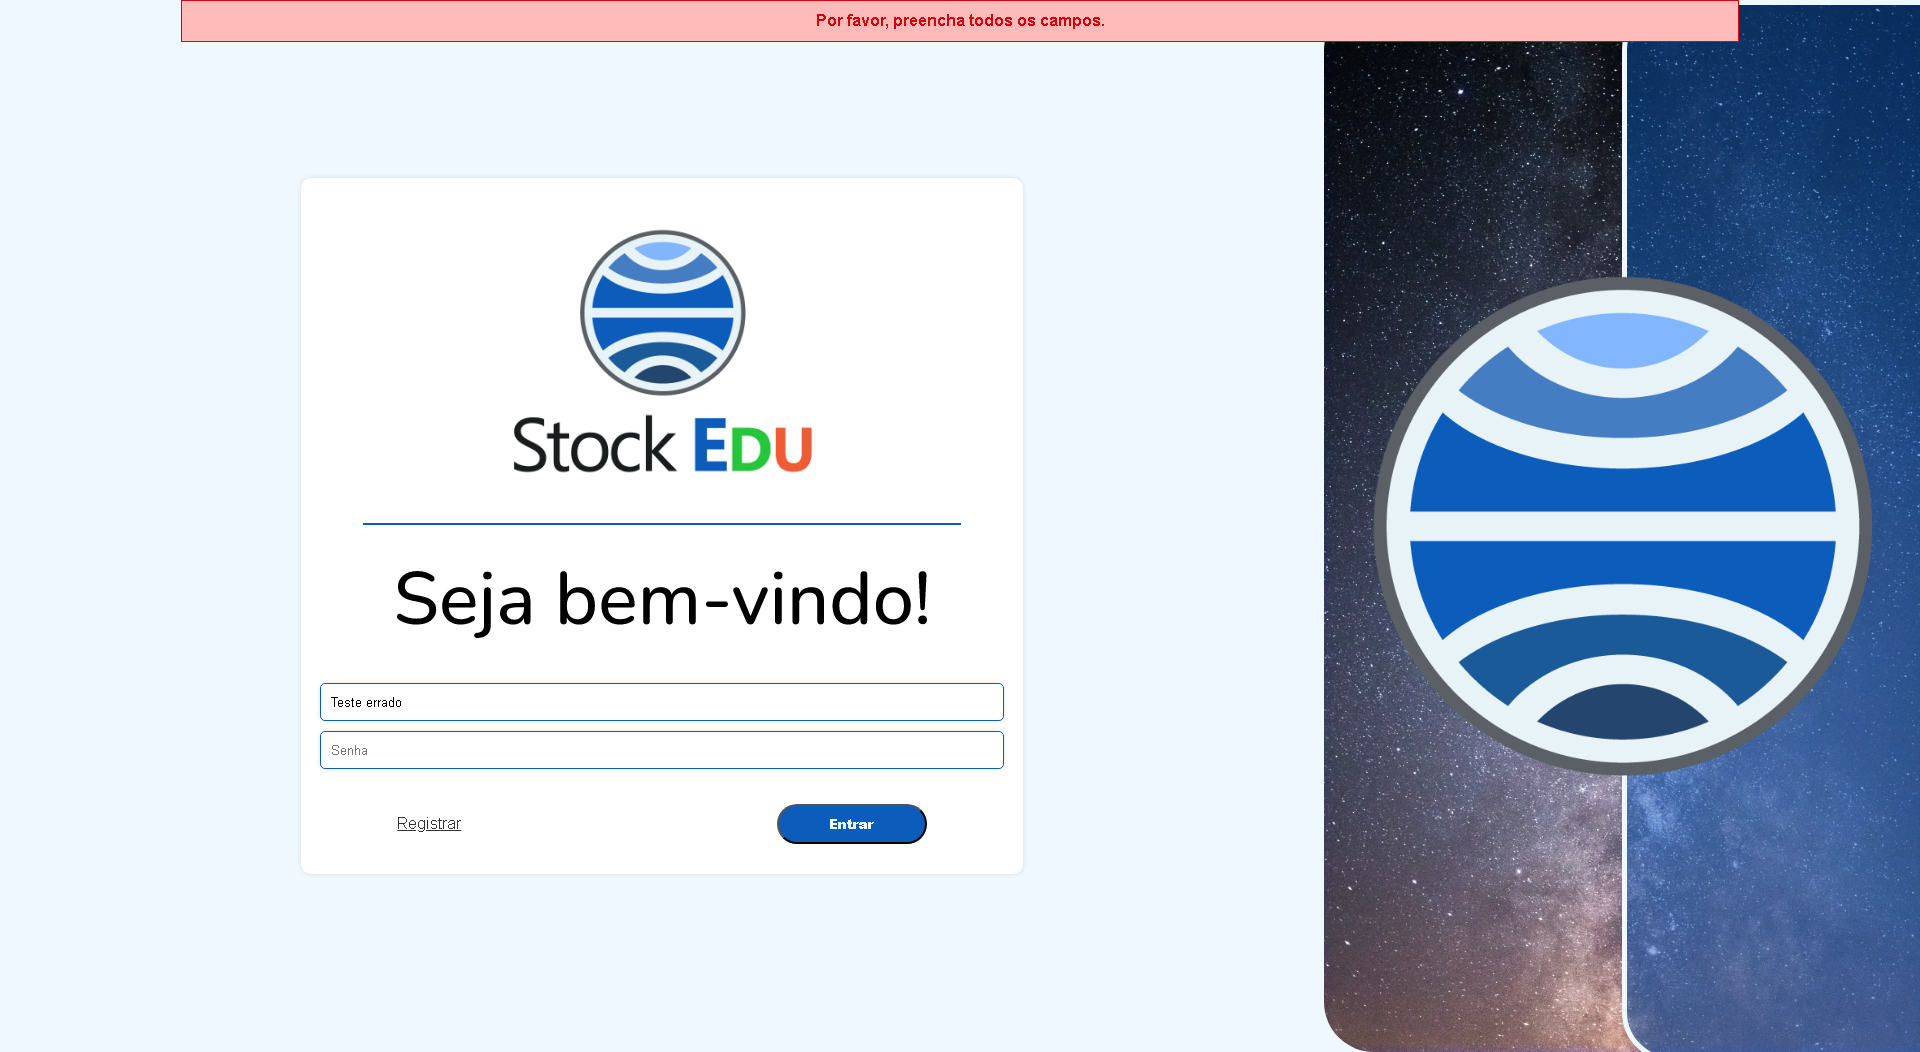
\includegraphics[width=0.6\textwidth]{fig/print2-errologin.png}
	\caption{Mensagem de erro 1 (fonte: o autor).}
	\label{fig:print2-errologin}
\end{figure}

Se o usuário não houver se cadastrado, poderá criar um novo perfil em "Registrar", onde será redirecionado a um pequeno formulário:

\begin{figure}[htb]
	\centering
	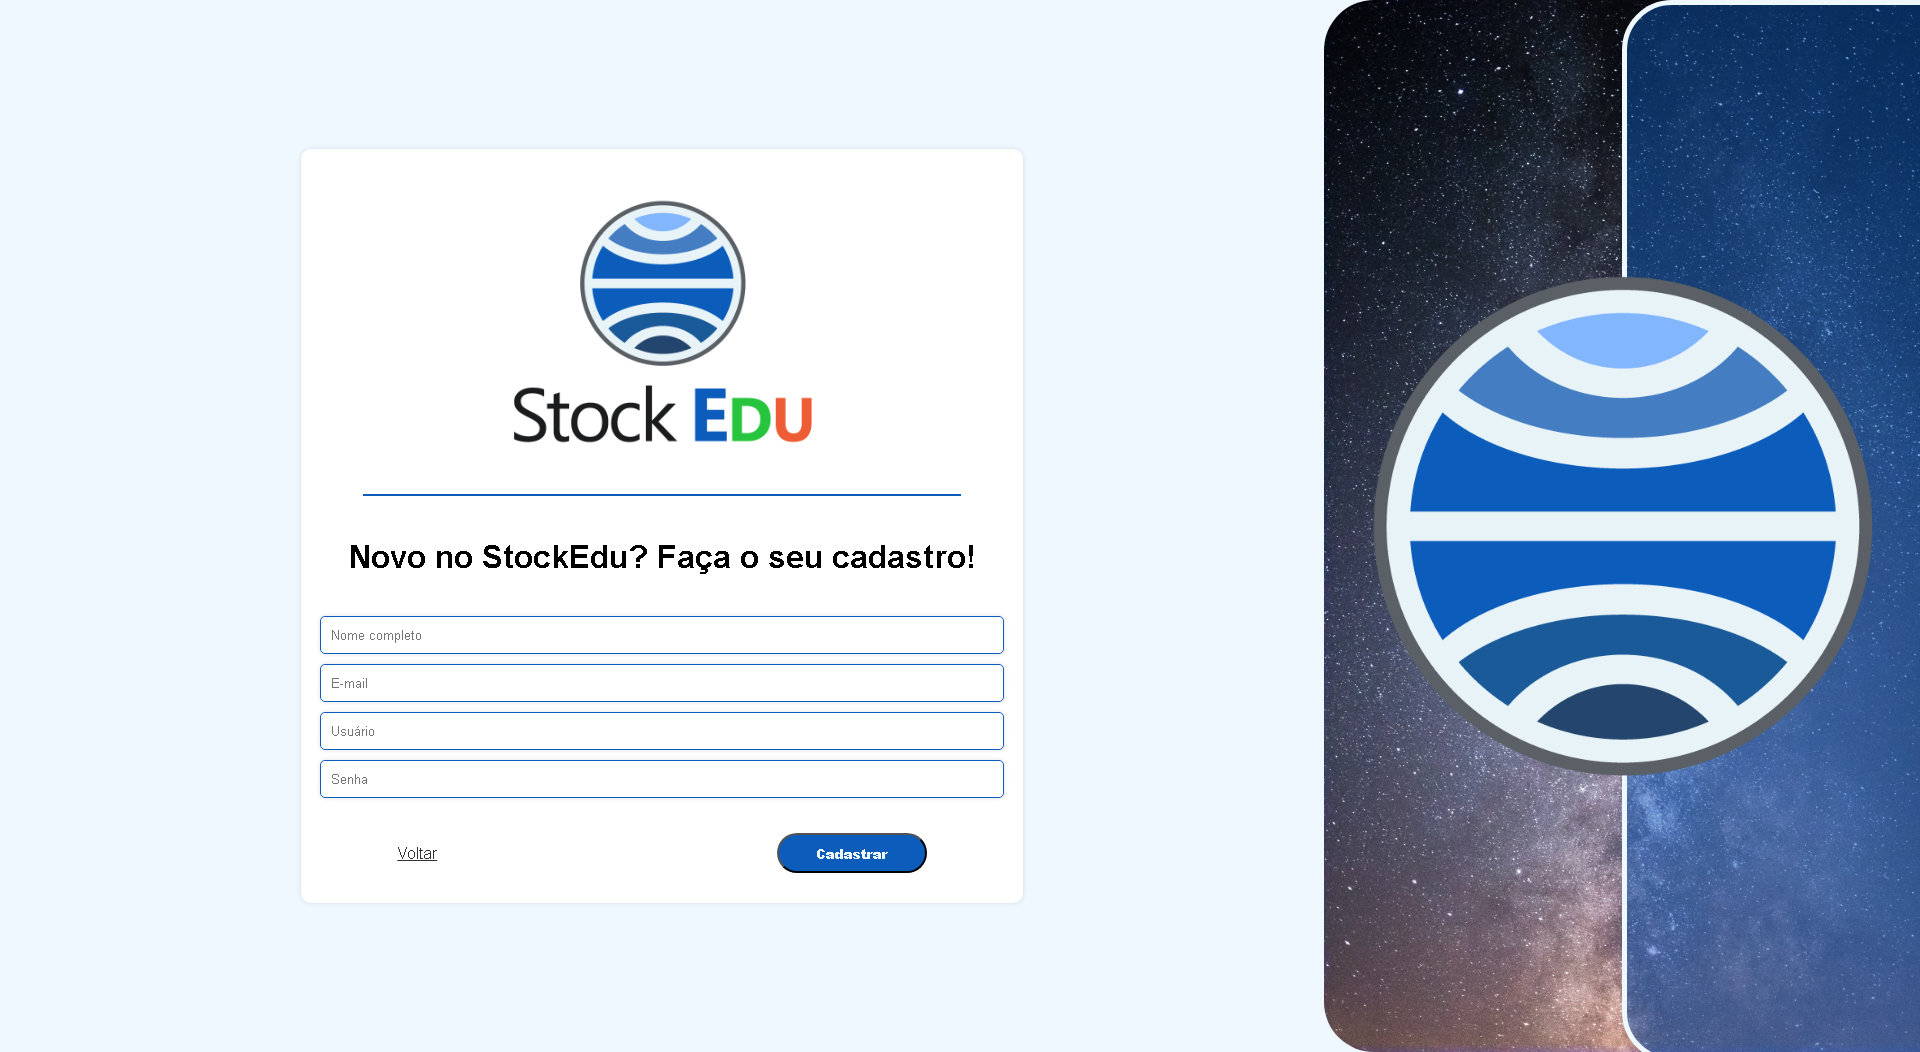
\includegraphics[width=0.6\textwidth]{fig/print3-cadastro.png}
	\caption{Tela de cadastro (fonte: o autor).}
	\label{fig:print3-cadastro}
\end{figure}

Caso o usuário preencher algum campo errado, uma mensagem de validação aparecerá apontando o erro. As validações aqui são para os seguintes casos:

\begin{enumerate}[label=\textbf{\Alph*)}]
	\item Email fora do padrão de ''xxxxxx@xxxx.com'';
	\item Nome de usuário já consta na base de dados;
	\item Senha fraca;
\end{enumerate}

Ao se cadastrar ou fazer o login corretamente, o usuário é redirecionado para a tela principal do aplicativo passando antes por uma tela de carregamento animada:

\begin{figure}[htb]
	\centering
	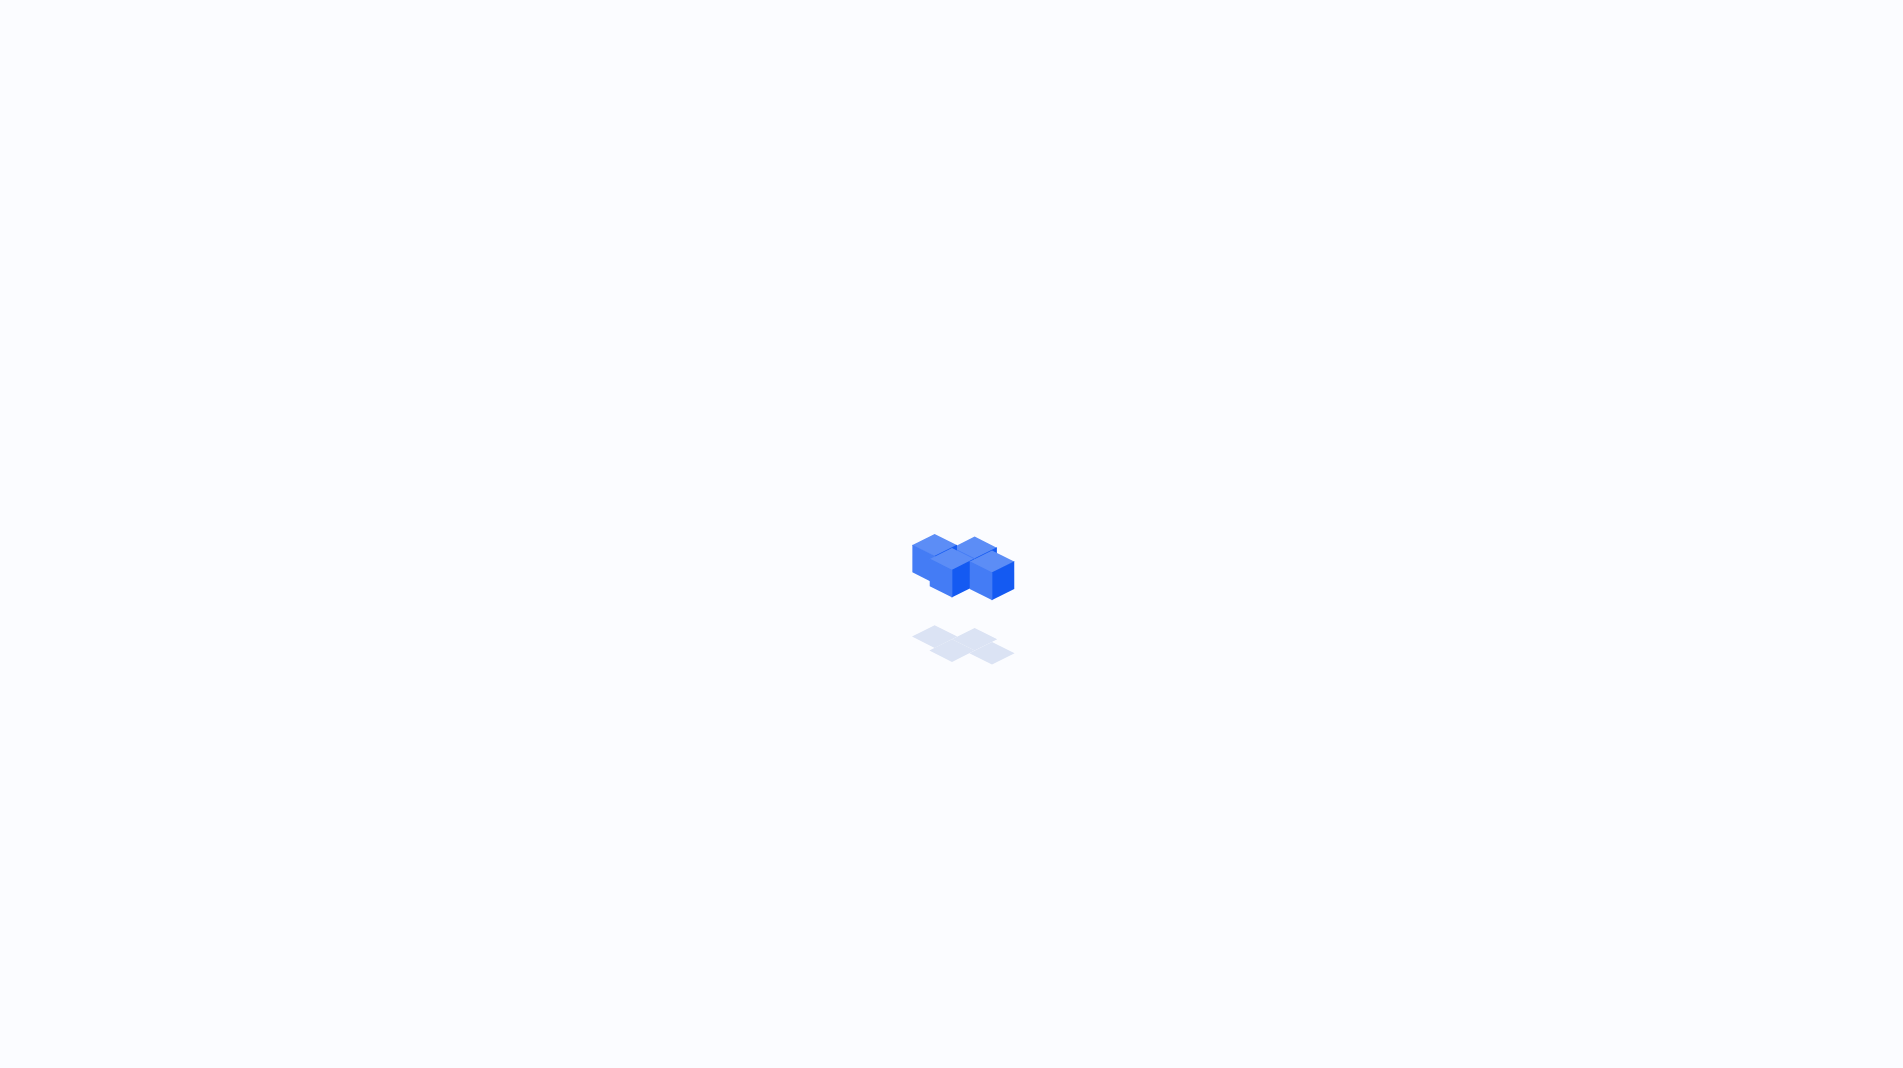
\includegraphics[width=0.6\textwidth]{fig/print4-teladecarregamento.png}
	\caption{Tela de carregamento (fonte: o autor).}
	\label{fig:print4-teladecarregamento}
\end{figure}

\begin{figure}[htb]
	\centering
	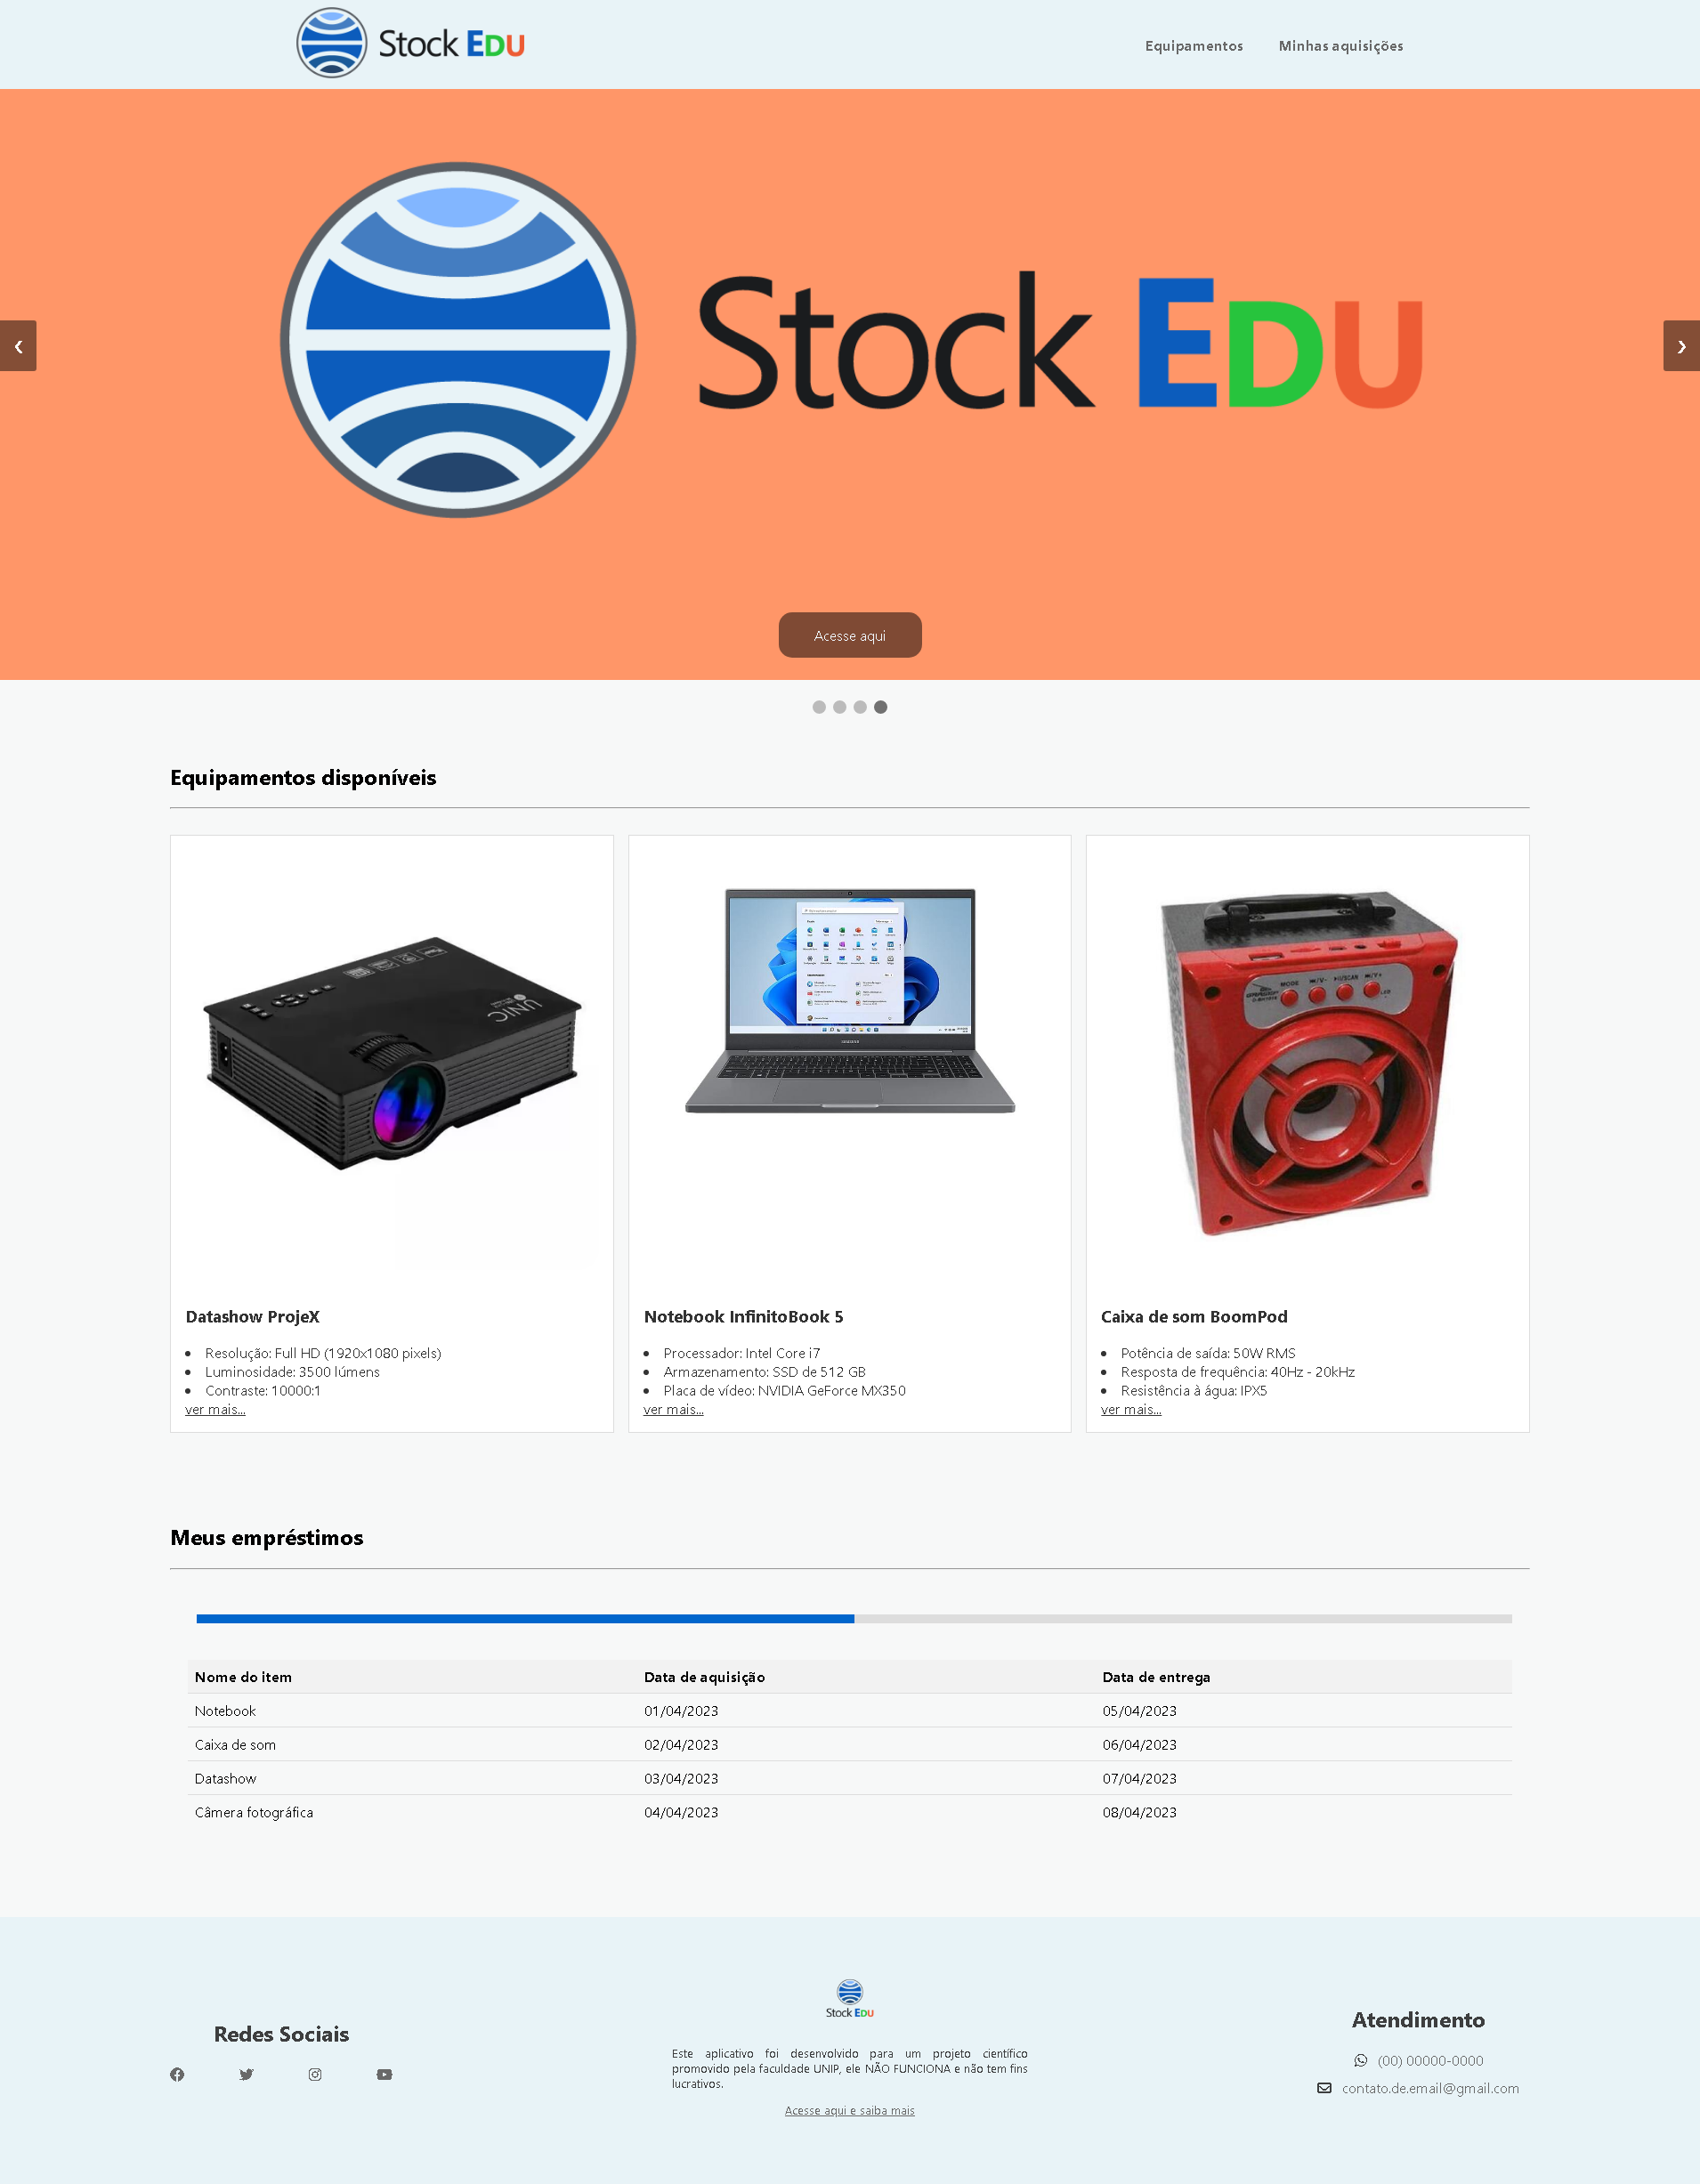
\includegraphics[width=0.6\textwidth]{fig/print5-telaprincipal.png}
	\caption{Tela principal (fonte: o autor).}
	\label{fig:print5-telaprincipal}
\end{figure}

Na tela principal há um slide de imagens completamente funcional com botões e um timer, uma prateleira de itens onde ficarão os itens cadastrados pela escola e uma área do usuário, onde haverá o histórico de empréstimos e solicitações, assim como as solicitações em aberto.

O cabeçalho da página contem botões com animações de rolagem e total responsividade:

\begin{figure}[htb]
	\centering
	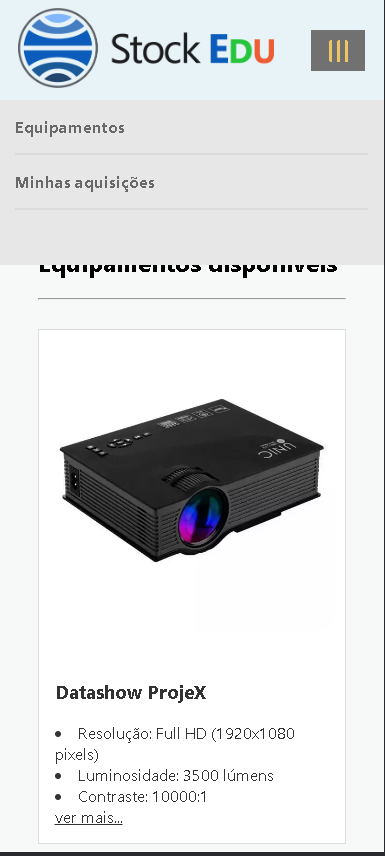
\includegraphics[width=0.4\textwidth]{fig/print6-responsividademain.png}
	\caption{Comportamento do cabeçalho em outros tamanhos de tela (fonte: o autor).}
	\label{fig:print6-responsividademain}
\end{figure}

O userflow da interface é bem definido e intuitivo. Ao acessar a tela inicial,
o usuário pode optar por navegar pelas seções de "Equipamentos" que atualmente
possui 3, uma caixa de som, um notebook e um projetor ou "Minhas Aquisições"
para verificar as movimentações que o usuário já realizou no sistema ao solicitar
equipamentos. Ao clicar na seção de "Equipamentos", é apresentada uma lista de
equipamentos disponíveis para empréstimo, com opções para saber mais sobre
cada equipamento e agendar o empréstimo.

\begin{figure}[htb]
	\centering
	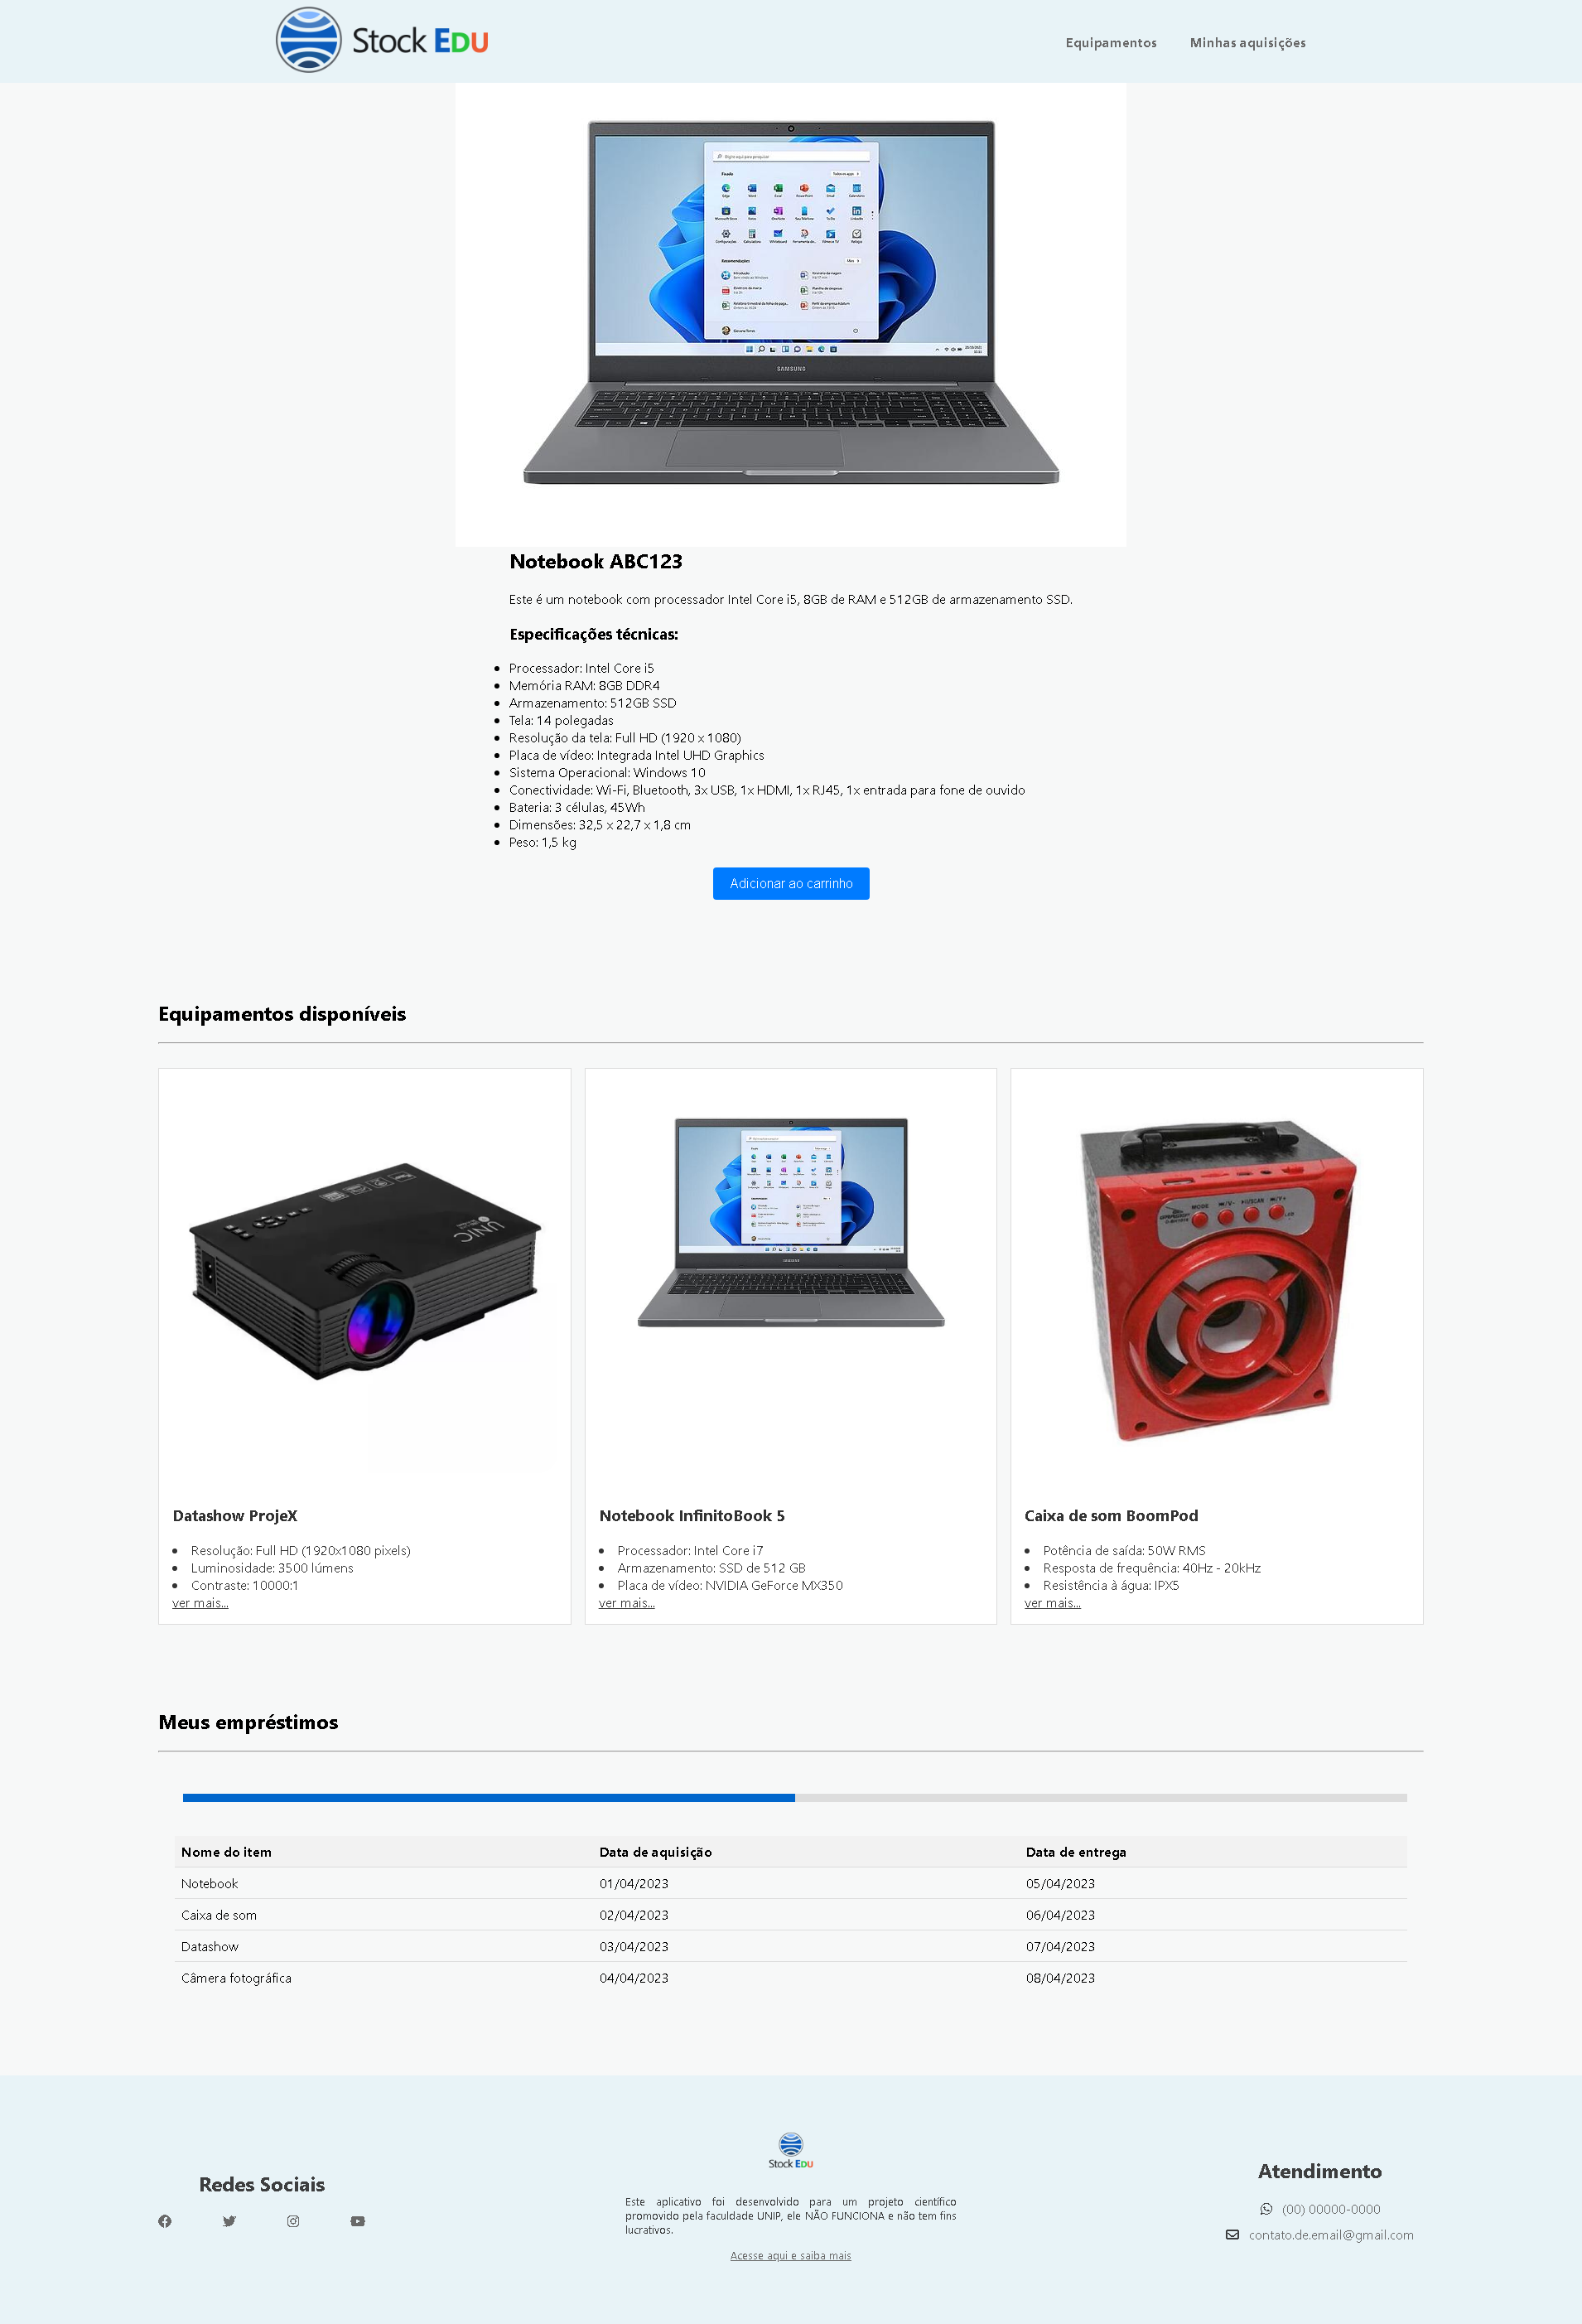
\includegraphics[width=0.4\textwidth]{fig/print7-telaproduto.png}
	\caption{Tela do item selecionado (fonte: o autor).}
	\label{fig:print7-telaproduto}
\end{figure}

A interface criada para o empréstimo de equipamentos audiovisuais para
escolas de ensino médio e fundamental apresenta uma estrutura bem definida, com
telas intuitivas e um userflow eficiente. O layout e a escolha dos elementos foram
coerentes com a temática da interface, o que ajuda a transmitir uma imagem
profissional e confiável da empresa. A logo da interface é simples e eficiente, com
um ícone de projetor que ajuda a identificar facilmente a atividade da empresa. No
geral, a interface é bem-sucedida em apresentar informações importantes de forma
clara e objetiva, além de permitir que os usuários realizem as ações desejadas de
forma fácil e intuitiva.


\chapter{Programação Orientada a Objetos}

A programação orientada a objetos proporciona um software com uma interface
atraente e fácil de usar. Ela utiliza conceitos do mundo real para representar
objetos, tornando a compreensão e a modificação do sistema mais fácil. Dessa
forma, a POO pode tornar a interface mais intuitiva para o usuário final. Essa
abordagem é benéfica para o desenvolvimento, reutilização de código,
encapsulamento e modularização, tornando essencial a utilização desses
conceitos técnicos.

No processo de criação de uma boa interface, é necessário entender alguns
elementos essenciais para exibir e manipular objetos no sistema de forma clara.
São eles as classes, que definem a estrutura do objeto, seus atributos e métodos,
além da interação com o usuário por meio de uma interface gráfica. Alguns dos
conceitos fundamentais da programação orientada a objetos são objetos, classes,
herança e polimorfismo.

Os objetos representam coisas reais ou abstratas que possuem atributos e
métodos. Por exemplo, um computador é um objeto com atributos como "marca"
e "modelo" e métodos como ligar, desligar, reiniciar e comandos. As classes
definem a estrutura do objeto e contêm informações necessárias para criá-lo,
como uma receita de bolo. A herança é responsável por "herdar" comportamentos
de outra classe, permitindo que um objeto tenha atributos e métodos da classe pai
e também adicionando características próprias. O polimorfismo ocorre quando
objetos de diferentes classes fazem a mesma função, mas de uma forma diferente.

Esses aspectos técnicos foram utilizados no código do projeto para garantir uma
estrutura clara e organizada, afim de facilitar e dinamizar a experiência final do
usuário. Neste trabalho, foi fundamental utilizar alguns conceitos, como a classe
"AparelhoAudiovisual" contendo atributos como "marca" e "modelo", ou a classe
"Projetor", que herda atributos e métodos da classe pai. Em resumo, a POO é
fundamental para criar programas mais organizados, eficientes e fáceis de manter.

% ----------------------------------------------------------
% Finaliza a parte no bookmark do PDF
% para que se inicie o bookmark na raiz
% e adiciona espaço de parte no Sumário
% ----------------------------------------------------------
\phantompart

\part{Conclusão}

% ---
% Conclusão
% ---
\chapter{Conclusão}
% ---

O colégio Vencer Sempre possuía um sistema antigo e pouco eficiente de
gerenciamento dos equipamentos, portanto o sistema feito para a escola foi
pensado não somente para facilitar sua distribuição como também para ser um
agregador na educação dos alunos uma vez que seus professores conseguirão
planejar melhor suas aulas, também foi pensado para garantir que as necessidades
do cliente sejam atendidas.



% ----------------------------------------------------------
% ELEMENTOS PÓS-TEXTUAIS
% ----------------------------------------------------------
\postextual
% ----------------------------------------------------------

% ----------------------------------------------------------
% Referências bibliográficas
% ----------------------------------------------------------
\bibliography{abntex2-modelo-references}

\begin{itemize}
    \item Alura. (s.d.). POO: Programação Orientada a Objetos, 2023 \\
	Disponível em: \url{https://www.alura.com.br/artigos/poo-programacao-orientada-aobjetos}
    \item FERREIRA, J. (s.d.). Aula 4 - Interfaces. Disponível em:\\
	\url{https://sites.google.com/site/anhangueraniteroipoo/aulas/aula-4---interfaces}
    \item CODIFICAR. (s.d.). Requisitos Funcionais e Não Funcionais: o que são e como
	identificá-los. Dísponivel em:\\ \url{https://codificar.com.br/requisitos-funcionais-naofuncionais/}
	\item DEV MEDIA. Revista Engenharia de Software
	\url{https://www.devmedia.com.br/introducaoa-engenharia-de-requisitos/8034}
	\item REDEQUISITOS. Quais os tipos de Requisitos de Software? Sabe a diferença
	entre eles?. Disponível em:\\
	\url{http://rederequisitos.com.br/quais-os-tipos-derequisitos-desoftware-sabe-diferenca-entre-eles/}
	\item REQUISITOS DE SISTEMA:\url{https://codificar.com.br/requisitos-funcionais-naofuncionais/#:~:text=Os%20requisitos%20funcionais%20descrevem%20o,qu}
	
\end{itemize}

%---------------------------------------------------------------------
% INDICE REMISSIVO
%---------------------------------------------------------------------
\phantompart
\printindex
%---------------------------------------------------------------------

\end{document}
